\section{Kiểm thử}
\textit{Sử dụng 10 testcase với ba đặc trưng khác nhau là: kích thước nhỏ, kích thước lớn, và không có đường đi.}

\subsection{Testcase với kích thước nhỏ}

\begin{figure}[H]
\centering
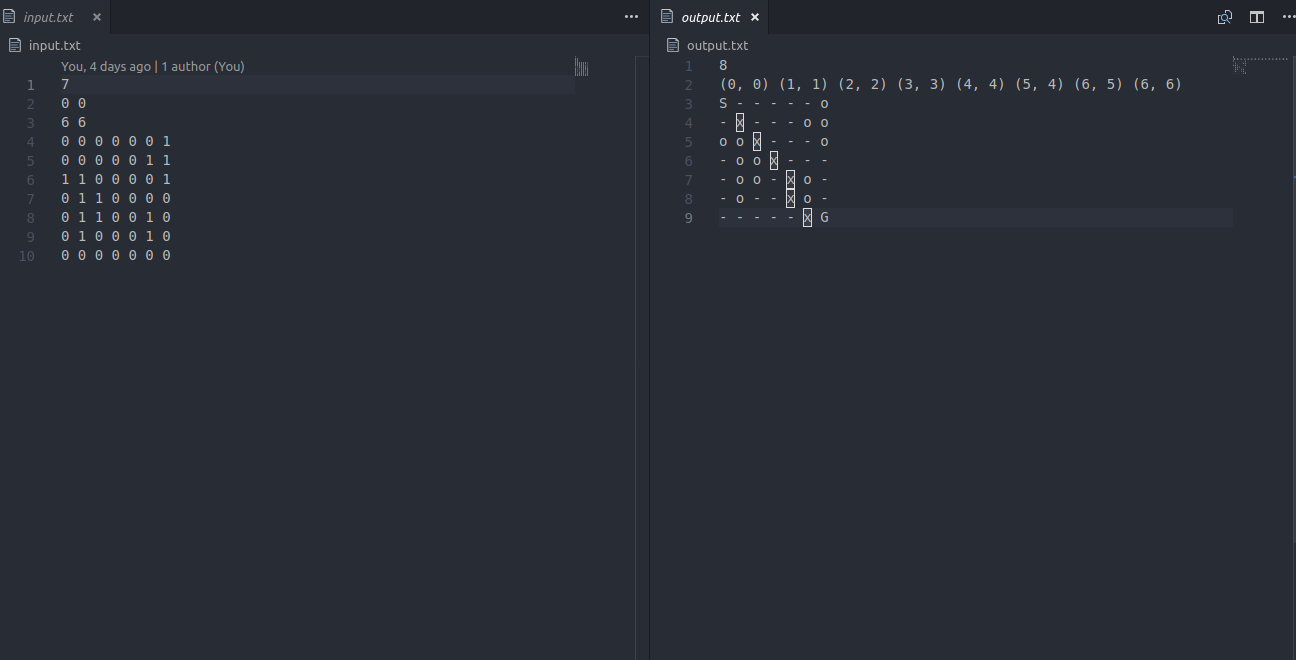
\includegraphics[width=0.98\textwidth]{t0.png}
\caption{Testcase 8x8.}
\end{figure}

\begin{figure}[H]
\centering
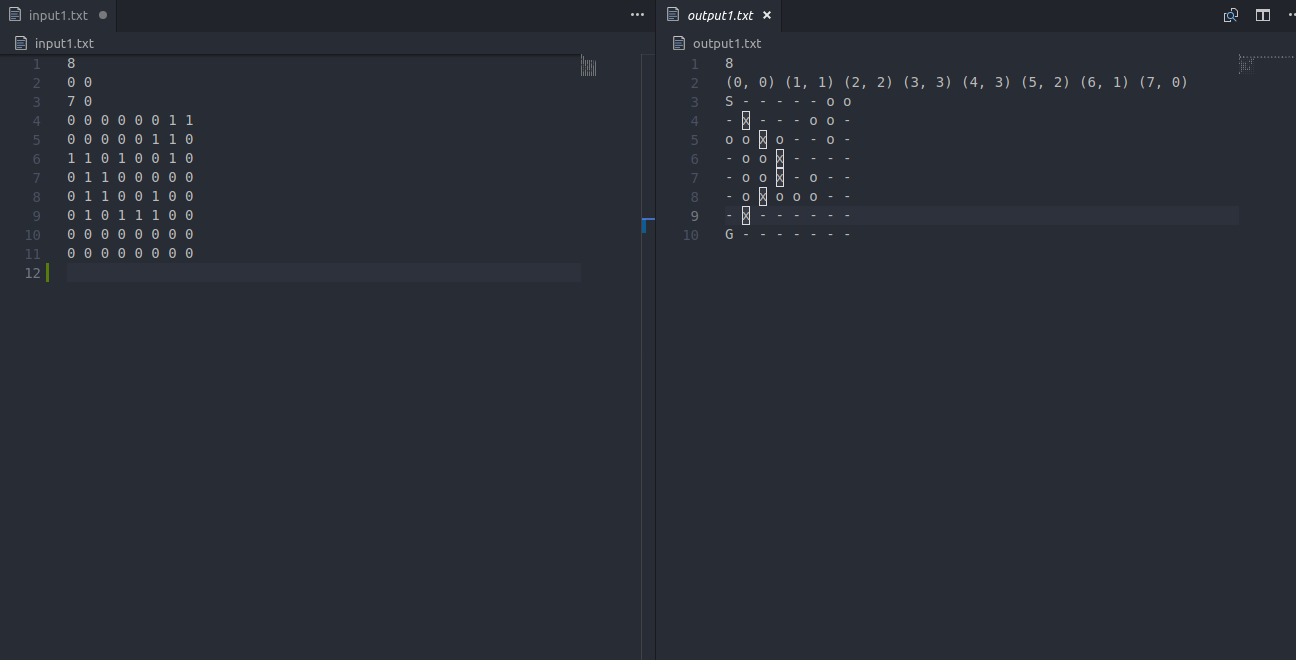
\includegraphics[width=0.98\textwidth]{t1.png}
\caption{Testcase 8x8.}
\end{figure}

\begin{figure}[H]
\centering
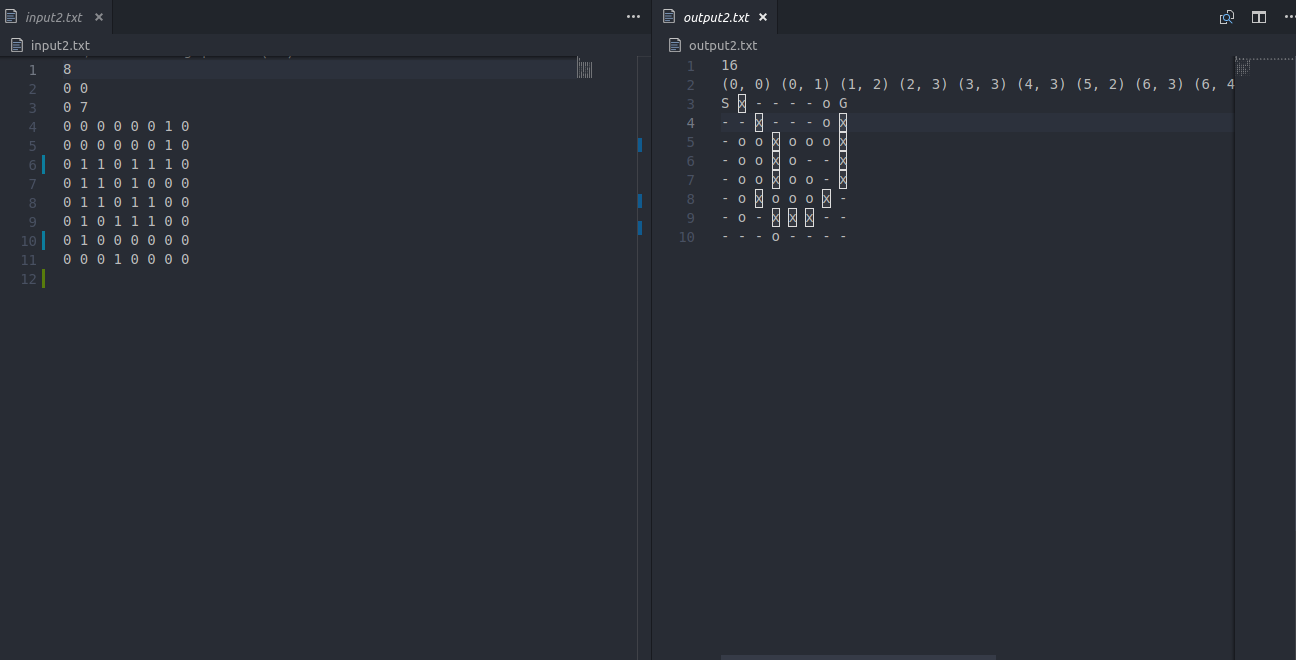
\includegraphics[width=0.98\textwidth]{t2.png}
\caption{Testcase 8x8.}
\end{figure}

\begin{figure}[H]
\centering
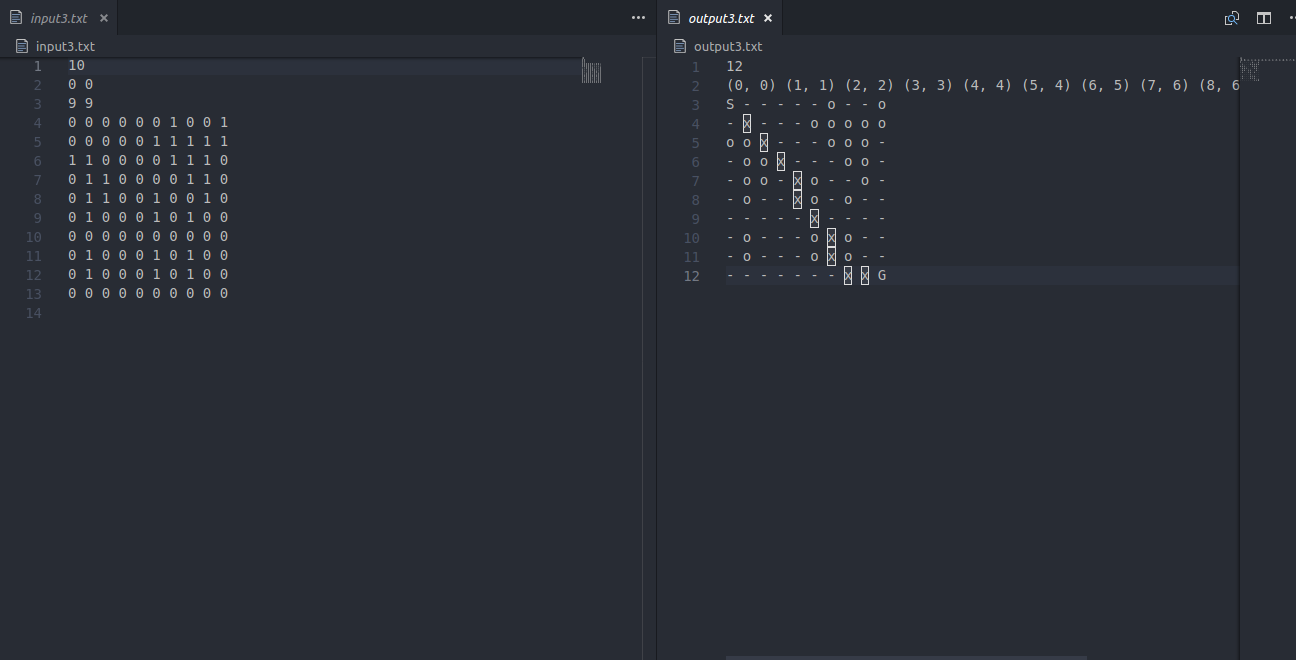
\includegraphics[width=0.98\textwidth]{t3.png}
\caption{Testcase 10x10.}
\end{figure}

\subsection{Testcase với kích thước lớn}

\begin{figure}[H]
\centering
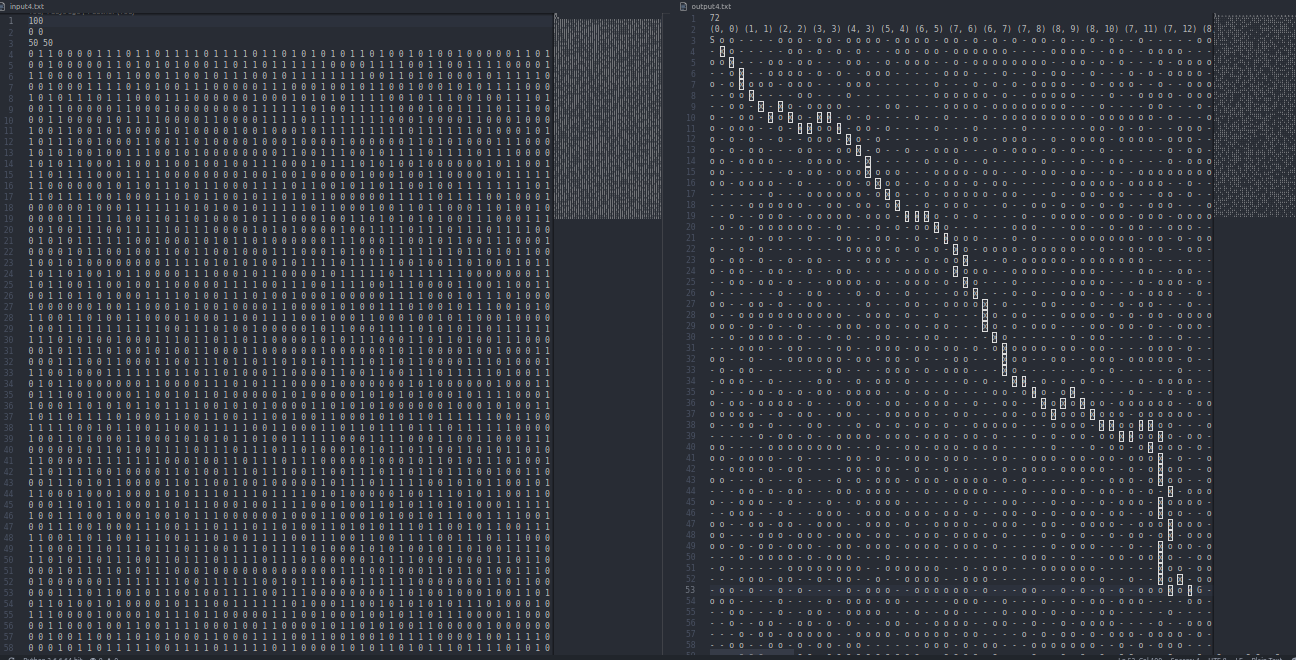
\includegraphics[width=0.98\textwidth]{t4.png}
\caption{Testcase 100x100.}
\end{figure}

\begin{figure}[H]
\centering
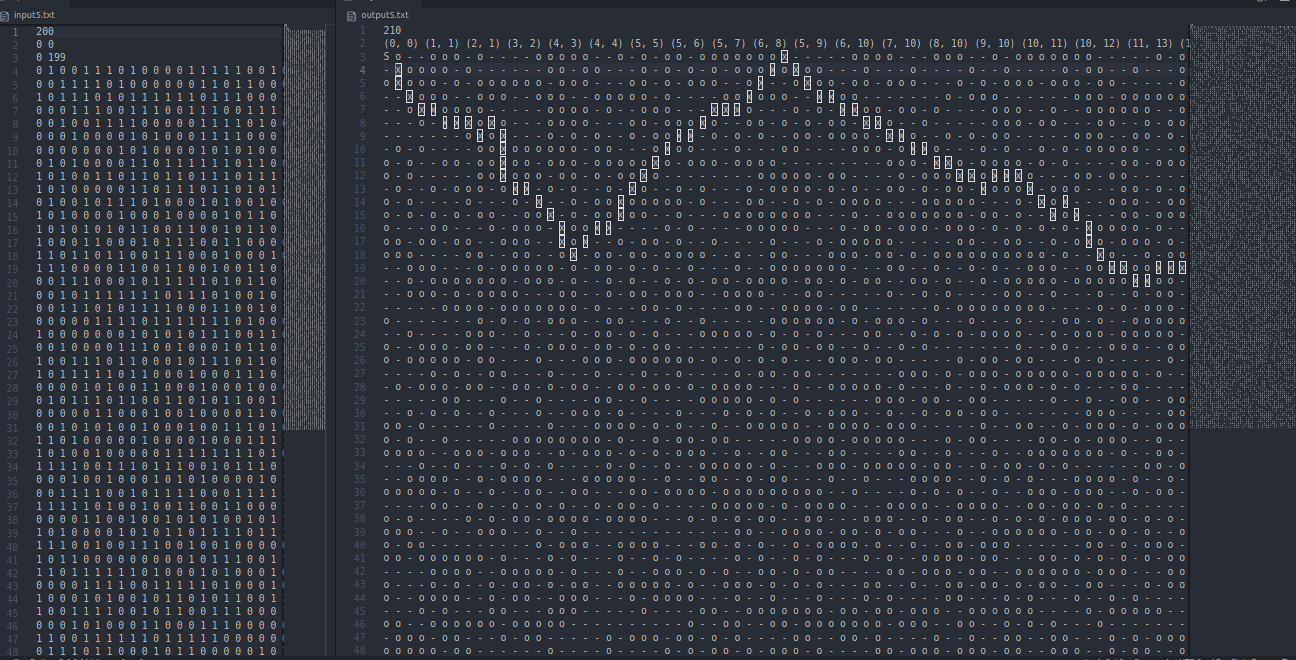
\includegraphics[width=0.98\textwidth]{t5.png}
\caption{Testcase 200x200.}
\end{figure}

\begin{figure}[H]
\centering
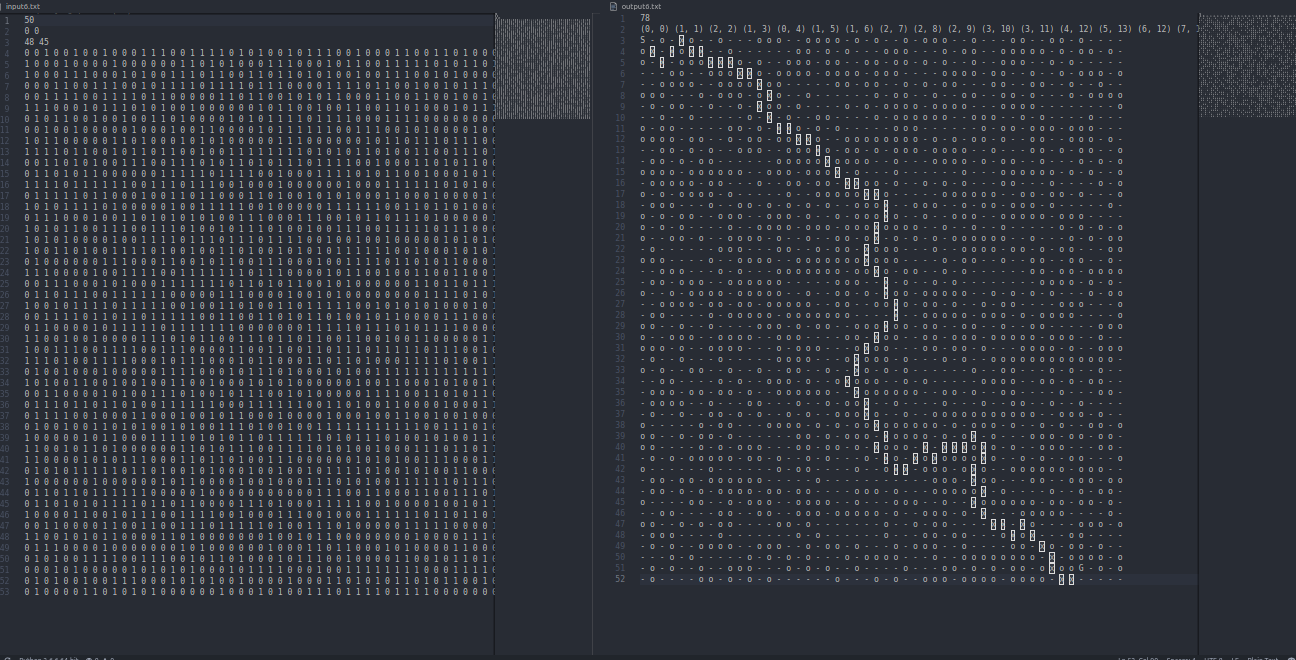
\includegraphics[width=0.98\textwidth]{t6.png}
\caption{Testcase 50x50.}
\end{figure}

\subsection{Testcase không có đường đi từ \code{start} đến \code{goal}}

\begin{figure}[H]
\centering
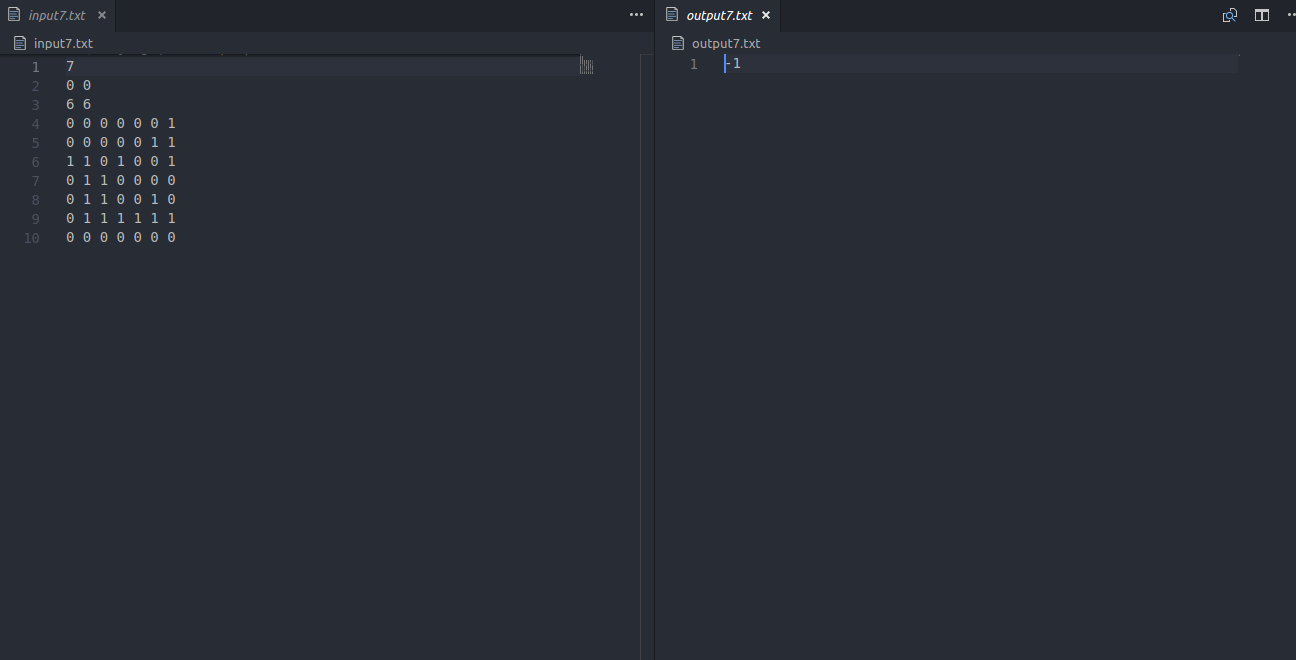
\includegraphics[width=0.98\textwidth]{t7.png}
\caption{Testcase 7x7.}
\end{figure}

\begin{figure}[H]
\centering
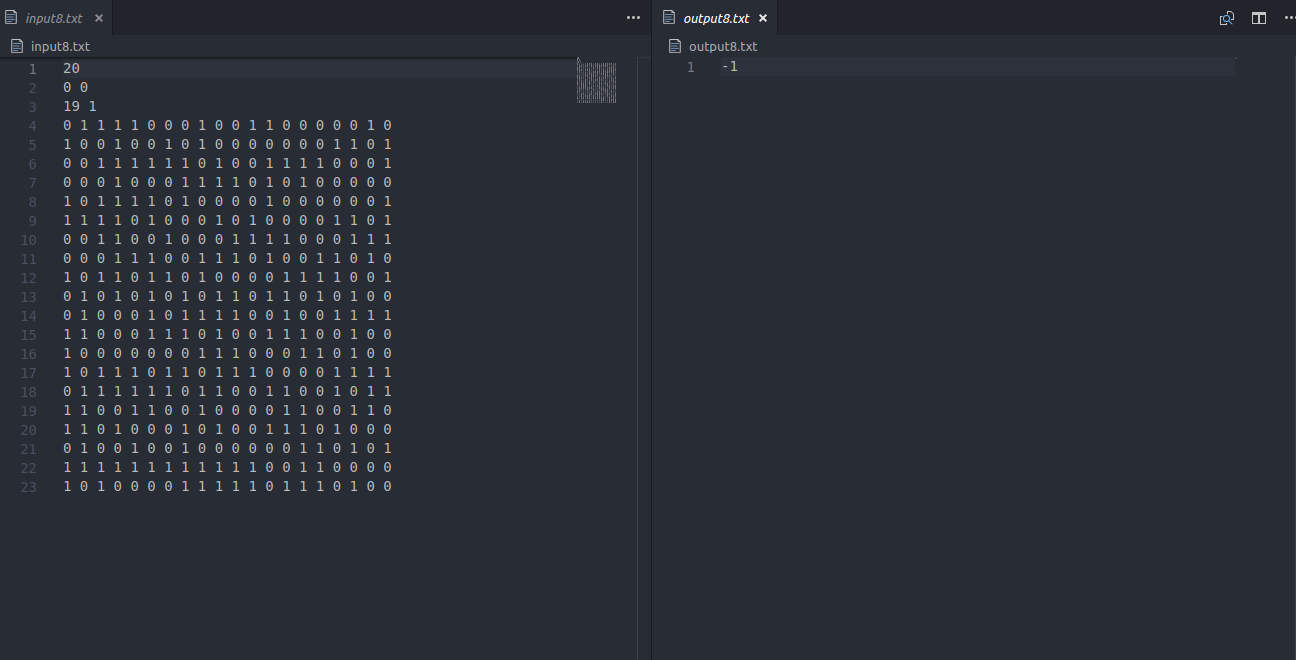
\includegraphics[width=0.98\textwidth]{t8.png}
\caption{Testcase 20x20.}
\end{figure}

\begin{figure}[H]
\centering
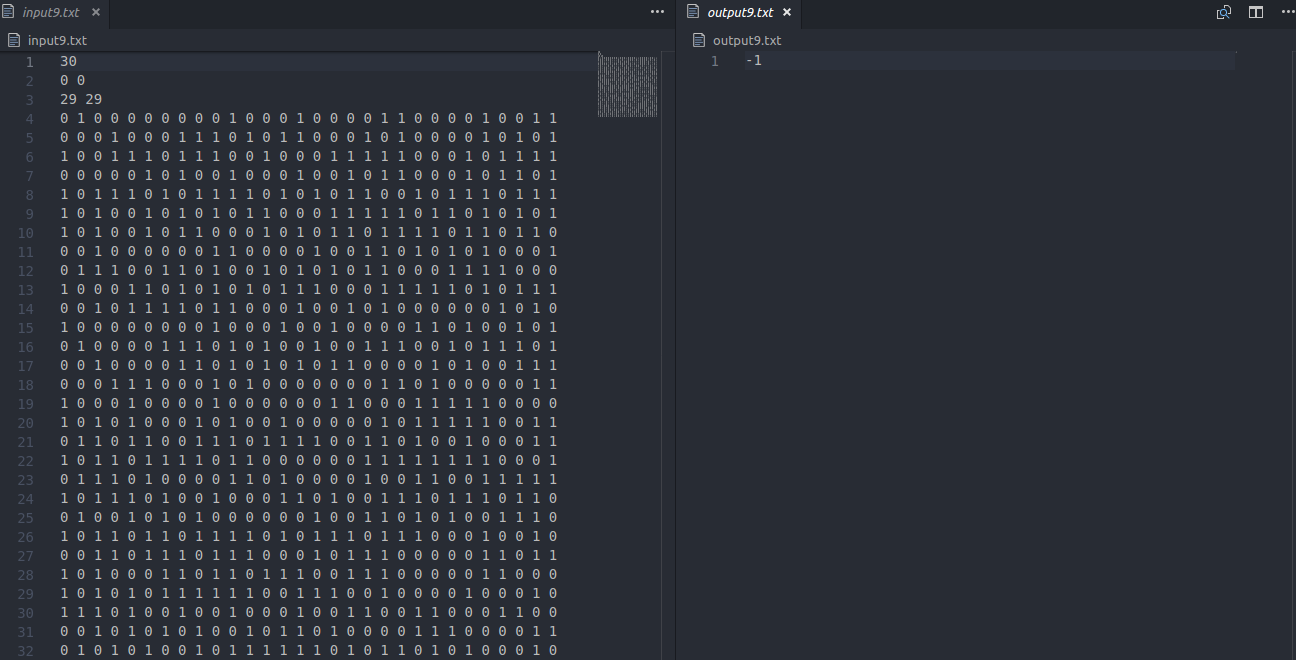
\includegraphics[width=0.98\textwidth]{t9.png}
\caption{Testcase 30x30.}
\end{figure}

\newpage